	
	On s'intéresse à la consommation d'essence d'un véhicule en fonction de sa vitesse.
	
	\subsection*{Lecture graphique}
	
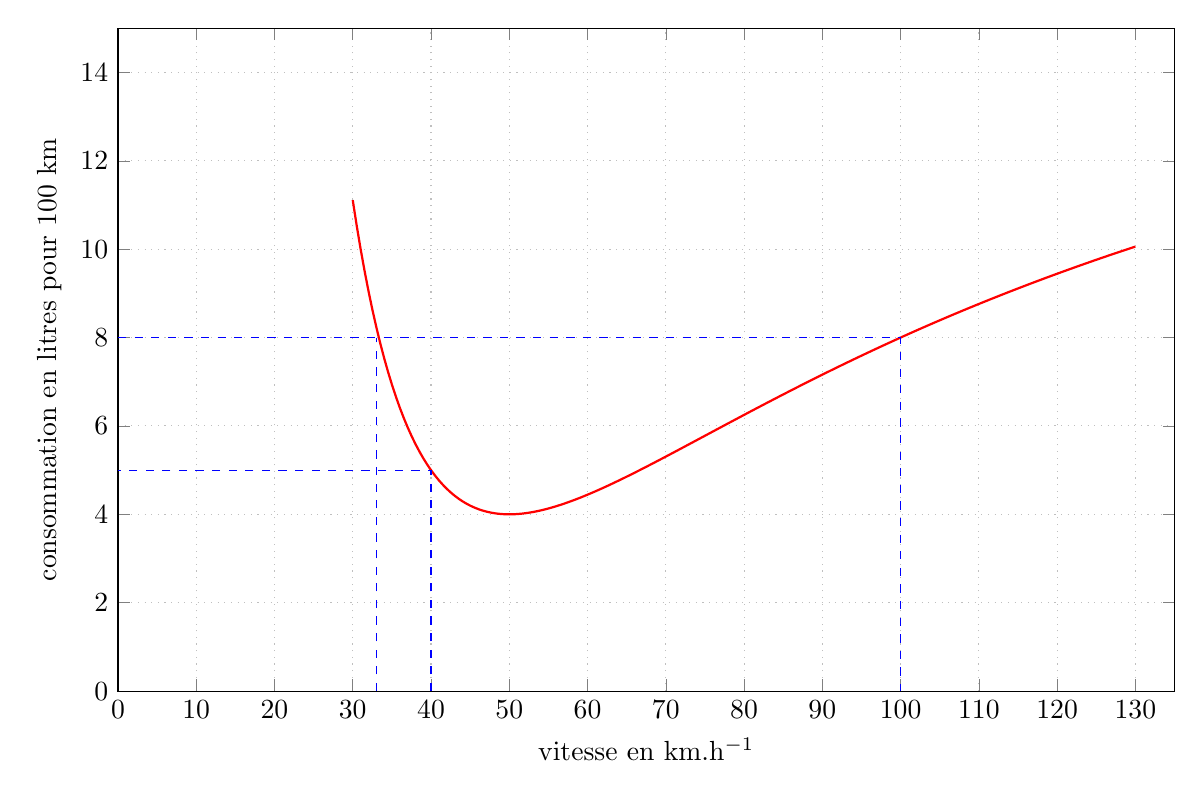
\begin{tikzpicture}
	\begin{axis}[
		width=15cm,
		height=10cm,
		grid=both,
		major grid style={dotted},
		xmajorgrids=true,
		ymajorgrids=true,
		xmin=0, xmax=135,
		ymin=0, ymax=15,
		xtick={0,10,...,135},
		ytick={0,2,...,14},
		xlabel={\text{vitesse en km.h$^{-1}$}},
		ylabel={\text{consommation en litres pour 100 km}}
		]
		\addplot[
		domain=30:130, 
		samples=200, 
		red, 
		thick
		] {20*x^2 - 1600*x + 40000)/(x^2)};
	\draw[dashed,blue](40,0)--(40,5)--(0,5);
	\draw[dashed,blue](0,8)--(100,8)--(100,0);
		\draw[dashed,blue](33,0)--(33,8);
	\end{axis}

\end{tikzpicture}

	\subsection*{1.}
	
	
	On lit environ 5 l.
	
	\subsection*{2.}
	

	On lit environ 33,3 km/h ou 100 km/h.
	
	\subsection*{3.}
	
	
	La consommation semble la plus basse à une vitesse de 50 km/h.
	
	\subsection*{4.}
	

	\(u\) et \(v\) étant deux fonctions dérivables et la dérivée de \(\dfrac{u}{v}\) (pour \(v \neq 0\)) étant \(\dfrac{u'v - uv'}{v^2}\), on a donc :
	
	\[ f'(x) = \dfrac{x^2 \times (40x - 1600) - 2x (20x^2 - 1600x + 40000)}{x^4} \]
	
	\[ = \dfrac{40x^3 - 1600x^2 - 40x^3 + 3200x^2 - 80000x}{x^4} \]
	
	\[ = \dfrac{1600x^2 - 80000x}{x^4} \]
	
	\[ = \dfrac{800(2x - 100)}{x^3} \]
	
	\subsection*{5.}
	
	
	On a \(800 > 0\) et on a aussi \(x^2 > 0\) quel que soit le réel \(x\), donc le signe de \(f'(x)\) est celui de la différence \(2x - 100\). Or :
	
	\begin{itemize}
		\item \(2x - 100 < 0 \iff 2x < 100 \iff x < 50\);
		\item \(2x - 100 > 0 \iff 2x > 100 \iff x > 50\);
		\item \(2x - 100 = 0 \iff 2x = 100 \iff x = 50\).
	\end{itemize}
	
	Du signe de la dérivée, on en déduit que \(f\) est décroissante pour \(x < 50\) et croissante pour \(x > 50\) :\\
	 \(f(50) = \dfrac{20 \times 50^2 - 1600 \times 50 + 40000}{50^2} = 36 - 32 = 4 \) est le minimum de la fonction.
	
